%% Courtney Gibbons, March 2025
%% No Triangles Math Activity for Kids by Courtney Gibbons is marked with CC0 1.0. 
%% To view a copy of this license, visit https://creativecommons.org/publicdomain/zero/1.0/
\documentclass{article}
\usepackage[margin = 1cm]{geometry}
\usepackage{standalone}
\usepackage{amsmath}
\usepackage{multicol}
    \setlength{\columnseprule}{.5pt}
\usepackage{graphics}
\usepackage{wrapfig}
\usepackage[inline]{enumitem}
\usepackage{tikz}
\usetikzlibrary{calc,intersections}

% \renewcommand{\arraystretch}{10}
\setlength\tabcolsep{2cm}


\pagestyle{empty}

\begin{document}
    
    \begin{huge} No Triangles! \end{huge} 
    \hfill 
    
\includegraphics[scale=.05]{No Triangles QR Code.png}

    \hrulefill

    \bigskip

    \begin{minipage}[b]{.7\textwidth}
        \begin{itemize}
            \item Rules (two players, two colors, one winner).
            \begin{itemize}
                \item You and your partner will use different colors.
                \item Taking turns, draw lines between the dots.
                \item The first person to make a triangle in their own color using 3 of the dots loses.
            \end{itemize}
            %
            \bigskip
            %
            \item Rules (two players, one color, one winner).
            \begin{itemize}
                \item You and your partner will use the \textbf{same color}.
                \item Taking turns, draw lines between the points.
                \item The first person to make a triangle using 3 of the points loses.
            \end{itemize}
            %
            \bigskip
            %
            \item Rules (two players, two colors, two winners).
            \begin{itemize}
                \item You and your partner will use different colors.
                \item Taking turns, draw lines between the points.
                \item If \textbf{either of you} makes a triangle with your own color, you both lose.
                \item If \textbf{neither of you} makes a triangle with your own color, you both win.
            \end{itemize}
        \end{itemize}
    \end{minipage}
    %
    \begin{minipage}[b]{.3\textwidth}
        \scalebox{.9}{
            \documentclass[tikz,border=10pt]{standalone}
\usepackage{tikz}
\usepackage{amsmath}
\usetikzlibrary{calc,intersections}

\begin{document}

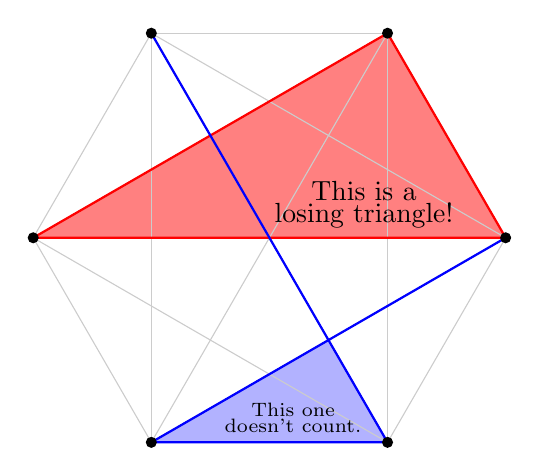
\begin{tikzpicture}
  % Define the radius of the hexagon
  \def\radius{3cm}

  % Define the vertices of the hexagon
  \foreach \i in {1,...,6} {
    \coordinate (V\i) at ({\radius*cos(60*(\i-1))}, {\radius*sin(60*(\i-1))});
  }

  % Name special paths
  \draw[name path=A] (V3)--(V6);
  \draw[name path=B] (V1)--(V5);

  % Define relevant intersection
  \path [name intersections={of=A and B,by=E}];

  % Create "Bad Triangle" region
  \draw[fill=blue!30!] (V6) -- (V5) -- (E) -- (V6);

  % Create "Good Triangle" region
  \draw[fill=red!50!] (V1) -- (V2) -- (V4) -- (V1);

  % Draw edges for the complete graph K6
  \foreach \i in {1,...,6} {
    \foreach \j in {\i,...,6} % slight improvement suggested by Japheth Wood
      \draw[black!20!] (V\i) -- (V\j);
    }

  % Draw special edges
` \draw[thick, red] (V1) -- (V2) -- (V4) -- (V1);
  \draw[thick, blue] (V3) -- (V6) -- (V5) -- (V1);

  % Draw the vertices
  \foreach \i in {1,...,6} {
    \fill (V\i) circle (2pt);
  }

  % Label good and bad triangles with text
  \node[above] at ($(V1)!0.3!(V4)$) {\Large $\substack{\text{This is a}\\\text{losing triangle!}}$};
  \node[above] at ($(V5)!0.6!(V6)$) {\normalsize $\substack{\text{This one}\\\text{doesn't count.}}$};

\end{tikzpicture}

\end{document}
        }
    \end{minipage}

    \hrulefill

    \bigskip
    \begin{Large}Mathematical Questions\end{Large}

    \begin{enumerate}
        \item Can you play No Triangles on a triangle? % yes but it's boring
        \item How many turns can a game of No Triangles last on a...\\ % answer following question before this one - talk about re-stating the question as a math strategy
        \begin{itemize*}
            \item ...square (4 dots)? \hspace{1cm} \phantom{1} %
            \item ...pentagon (5 dots)? \hspace{1cm} \phantom{1} %
            \item ...hexagon (6 dots)? \hspace{1cm} \phantom{1} %
            \item ...heptagon (7 dots)? \hspace{1cm} %
        \end{itemize*}
        \item In a game of No Triangles, how many lines are there for you and your partner to draw on a...\\
        \begin{itemize*}
            \item ...square (4 dots)? \hspace{1cm} \phantom{1} %
            \item ...pentagon (5 dots)? \hspace{1cm} \phantom{1} % 4 + 3 + 2 + 1 + 0 = 10
            \item ...hexagon (6 dots)? \hspace{1cm} \phantom{1} % 5 + 4 + 3 + 2 + 1 + 0 = 15
            \item ...heptagon (7 dots)? % 6 + 5 + 4 + 3 + 2 + 1 + 0 = 21
        \end{itemize*}
        \item Is there a ``good'' way to count the lines? 
        % strategy 1: count on a square; add one dot and add the new lines you need (repeat); 
        % strategy 2: start at a dot and count the (n-1) lines from it; the next dot has (n-1) too, but you already counted one, so there are only (n-2) that you haven't counted
        % strategy 3 (older kids): explain what $\binom{n}{2}$ is and how to figure out the formula
        \item In a game of No Triangles, how many possible triangles are there on a...\\
        \begin{itemize*}
            \item ...square (4 dots)? \hspace{1cm} \phantom{1} %
            \item ...pentagon (5 dots)? \hspace{1cm} \phantom{1}
            \item ...hexagon (6 dots)? \hspace{1cm} \phantom{1}
            \item ...heptagon (7 dots)?
        \end{itemize*}
        \item Is there a ``good'' way to count the triangles?
        % strategy 1: for each line, figure out how many triangles it's part of (n-2),
        % then multiply by the number of lines (see earlier)
        % then divide by 3 because you counted each triangle three times!
        % strategy 2: see if they can figure out that the answer must be $\binom{n}{3}$ if you used binomial coefficients earlier
        \item Can a game of No Triangles (two players, two colors, one winner) end in a tie (no winner) on a...\\
        \begin{itemize*}
            \item ...square (4 dots)? \hspace{1cm} \phantom{1} %
            \item ...pentagon (5 dots)? \hspace{1cm} \phantom{1} % yes, have them find one
            \item ...hexagon (6 dots)? \hspace{1cm} \phantom{1} % yes, have them find one % no, the best you can do is 14 turns without a triangle; see if they can find a 14 move tie
            \item ...heptagon (7 dots)?
        \end{itemize*}
        \item What about the other versions of No Triangles? Can they end without a winner?
        \item A third friend wants to play (three players, three colors, one winner). How many dots do you need for the game to be fun?
        \item Your friend makes a triangle, but you don't notice. Then, on your turn, you make a triangle---but you also notice the triangle your friend just made. How do you decide who wins?
        \item In the pictures up above, one game had a triangle that didn't count. What if you change the rules to \textit{also} count triangles with a point or points where lines intersect? How many triangles does a square, (or pentagon, or hexagon, or heptagon) have with these new rules?
        \item Can you come up your own version(s) of a No Shapes game?
    \end{enumerate}

    \clearpage
    %
    \begin{center}
        \begin{tabular}{c | c}
        %
            \documentclass[tikz,border=10pt]{standalone}
\usepackage{tikz}
\usetikzlibrary{calc}

\begin{document}

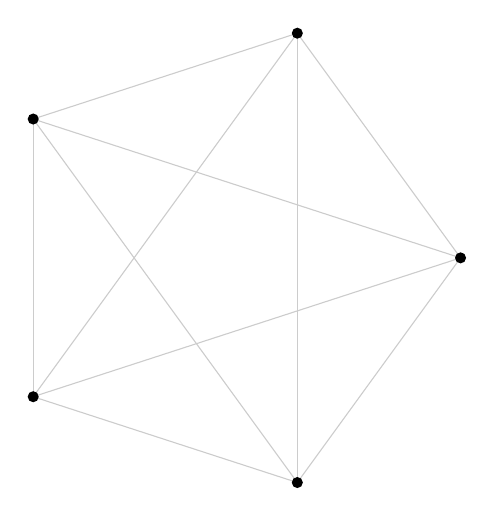
\begin{tikzpicture}
  % Define the radius of the hexagon
  \def\radius{3cm}

  % Define the vertices of the hexagon
  \foreach \i in {1,...,5} {
    \coordinate (V\i) at ({\radius*cos(72*(\i-1))}, {\radius*sin(72*(\i-1))});
  }

  % Draw edges for the complete graph K6
  \foreach \i in {1,...,5} {
    \foreach \j in {\i,...,5} % slight improvement suggested by Japheth Wood
      \draw[black!20!] (V\i) -- (V\j);
    }

  % Draw the vertices
  \foreach \i in {1,...,5} {
    \fill (V\i) circle (2pt);
  }

\end{tikzpicture}

\end{document} & \documentclass[tikz,border=10pt]{standalone}
\usepackage{tikz}
\usetikzlibrary{calc}

\begin{document}

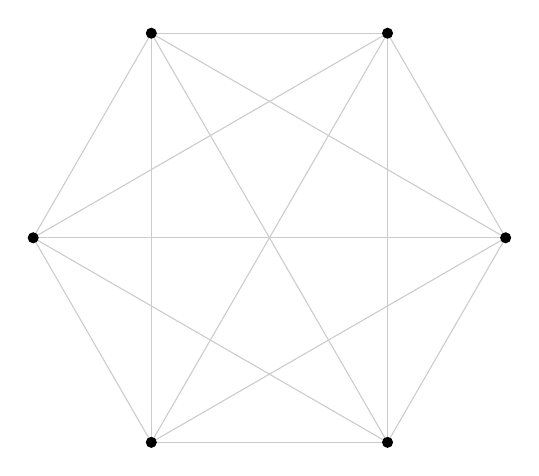
\begin{tikzpicture}
  % Define the radius of the hexagon
  \def\radius{3cm}

  % Define the vertices of the hexagon
  \foreach \i in {1,...,6} {
    \coordinate (V\i) at ({\radius*cos(60*(\i-1))}, {\radius*sin(60*(\i-1))});
  }

  % Draw edges for the complete graph K6
  \foreach \i in {1,...,6} {
    \foreach \j in {\i,...,6} % slight improvement suggested by Japheth Wood
      \draw[black!20!] (V\i) -- (V\j);
    }

  % Draw the vertices
  \foreach \i in {1,...,6} {
    \fill (V\i) circle (2pt);
  }

\end{tikzpicture}

\end{document} \\[1cm]
            \hline\\[1cm]
            \documentclass[tikz,border=10pt]{standalone}
\usepackage{tikz}
\usetikzlibrary{calc}

\begin{document}

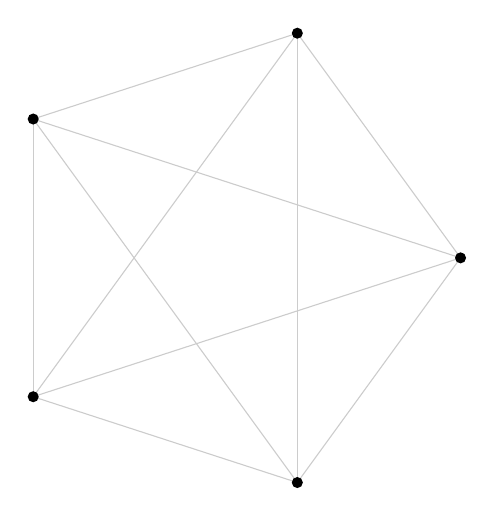
\begin{tikzpicture}
  % Define the radius of the hexagon
  \def\radius{3cm}

  % Define the vertices of the hexagon
  \foreach \i in {1,...,5} {
    \coordinate (V\i) at ({\radius*cos(72*(\i-1))}, {\radius*sin(72*(\i-1))});
  }

  % Draw edges for the complete graph K6
  \foreach \i in {1,...,5} {
    \foreach \j in {\i,...,5} % slight improvement suggested by Japheth Wood
      \draw[black!20!] (V\i) -- (V\j);
    }

  % Draw the vertices
  \foreach \i in {1,...,5} {
    \fill (V\i) circle (2pt);
  }

\end{tikzpicture}

\end{document} & \documentclass[tikz,border=10pt]{standalone}
\usepackage{tikz}
\usetikzlibrary{calc}

\begin{document}

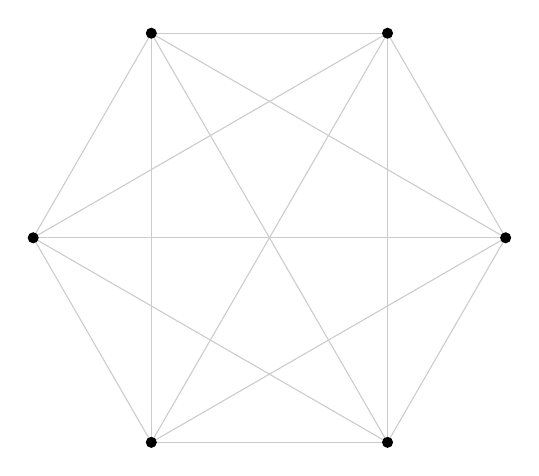
\begin{tikzpicture}
  % Define the radius of the hexagon
  \def\radius{3cm}

  % Define the vertices of the hexagon
  \foreach \i in {1,...,6} {
    \coordinate (V\i) at ({\radius*cos(60*(\i-1))}, {\radius*sin(60*(\i-1))});
  }

  % Draw edges for the complete graph K6
  \foreach \i in {1,...,6} {
    \foreach \j in {\i,...,6} % slight improvement suggested by Japheth Wood
      \draw[black!20!] (V\i) -- (V\j);
    }

  % Draw the vertices
  \foreach \i in {1,...,6} {
    \fill (V\i) circle (2pt);
  }

\end{tikzpicture}

\end{document} \\[1cm]
            \hline\\[1cm]
            \documentclass[tikz,border=10pt]{standalone}
\usepackage{tikz}
\usetikzlibrary{calc}

\begin{document}

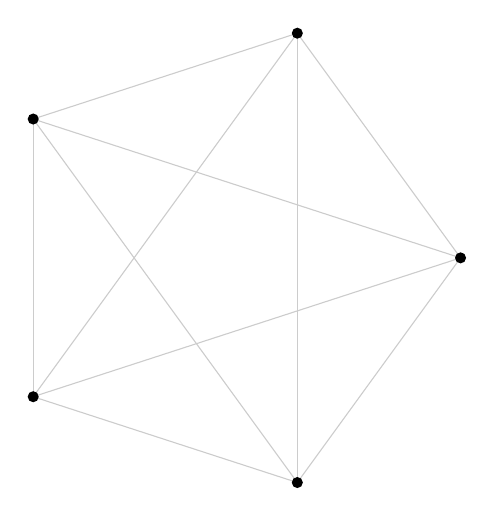
\begin{tikzpicture}
  % Define the radius of the hexagon
  \def\radius{3cm}

  % Define the vertices of the hexagon
  \foreach \i in {1,...,5} {
    \coordinate (V\i) at ({\radius*cos(72*(\i-1))}, {\radius*sin(72*(\i-1))});
  }

  % Draw edges for the complete graph K6
  \foreach \i in {1,...,5} {
    \foreach \j in {\i,...,5} % slight improvement suggested by Japheth Wood
      \draw[black!20!] (V\i) -- (V\j);
    }

  % Draw the vertices
  \foreach \i in {1,...,5} {
    \fill (V\i) circle (2pt);
  }

\end{tikzpicture}

\end{document} & \documentclass[tikz,border=10pt]{standalone}
\usepackage{tikz}
\usetikzlibrary{calc}

\begin{document}

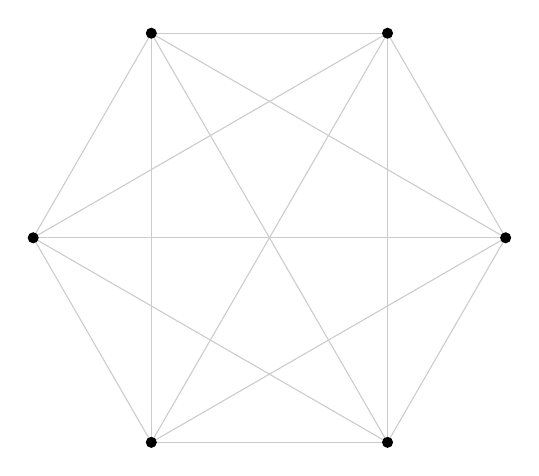
\begin{tikzpicture}
  % Define the radius of the hexagon
  \def\radius{3cm}

  % Define the vertices of the hexagon
  \foreach \i in {1,...,6} {
    \coordinate (V\i) at ({\radius*cos(60*(\i-1))}, {\radius*sin(60*(\i-1))});
  }

  % Draw edges for the complete graph K6
  \foreach \i in {1,...,6} {
    \foreach \j in {\i,...,6} % slight improvement suggested by Japheth Wood
      \draw[black!20!] (V\i) -- (V\j);
    }

  % Draw the vertices
  \foreach \i in {1,...,6} {
    \fill (V\i) circle (2pt);
  }

\end{tikzpicture}

\end{document} \\[1cm]
        \end{tabular}
    \end{center}
    %
    \clearpage
    %
    \begin{center}
        \begin{tabular}{c | c}
        %
            \documentclass[tikz,border=10pt]{standalone}
\usepackage{tikz}
\usetikzlibrary{calc}

\begin{document}

\begin{tikzpicture}
  % Define the radius of the hexagon
  \def\radius{3cm}

  % Define the vertices of the hexagon
  \foreach \i in {1,...,5} {
    \coordinate (V\i) at ({\radius*cos(72*(\i-1))}, {\radius*sin(72*(\i-1))});
  }

  % Draw the vertices
  \foreach \i in {1,...,5} {
    \fill (V\i) circle (2pt);
  }

\end{tikzpicture}

\end{document} & \documentclass[tikz,border=10pt]{standalone}
\usepackage{tikz}
\usetikzlibrary{calc}

\begin{document}

\begin{tikzpicture}
  % Define the radius of the hexagon
  \def\radius{3cm}

  % Define the vertices of the hexagon
  \foreach \i in {1,...,6} {
    \coordinate (V\i) at ({\radius*cos(60*(\i-1))}, {\radius*sin(60*(\i-1))});
  }

  % % Draw edges for the complete graph K6
  % \foreach \i in {1,...,6} {
  %   \foreach \j in {1,...,6}
  %     \draw[black!10!] (V\i) -- (V\j);
  %   }

  % Draw the vertices
  \foreach \i in {1,...,6} {
    \fill (V\i) circle (2pt);
  }

\end{tikzpicture}

\end{document} \\[1cm]
            \hline\\[1cm]
            \documentclass[tikz,border=10pt]{standalone}
\usepackage{tikz}
\usetikzlibrary{calc}

\begin{document}

\begin{tikzpicture}
  % Define the radius of the hexagon
  \def\radius{3cm}

  % Define the vertices of the hexagon
  \foreach \i in {1,...,5} {
    \coordinate (V\i) at ({\radius*cos(72*(\i-1))}, {\radius*sin(72*(\i-1))});
  }

  % Draw the vertices
  \foreach \i in {1,...,5} {
    \fill (V\i) circle (2pt);
  }

\end{tikzpicture}

\end{document} & \documentclass[tikz,border=10pt]{standalone}
\usepackage{tikz}
\usetikzlibrary{calc}

\begin{document}

\begin{tikzpicture}
  % Define the radius of the hexagon
  \def\radius{3cm}

  % Define the vertices of the hexagon
  \foreach \i in {1,...,6} {
    \coordinate (V\i) at ({\radius*cos(60*(\i-1))}, {\radius*sin(60*(\i-1))});
  }

  % % Draw edges for the complete graph K6
  % \foreach \i in {1,...,6} {
  %   \foreach \j in {1,...,6}
  %     \draw[black!10!] (V\i) -- (V\j);
  %   }

  % Draw the vertices
  \foreach \i in {1,...,6} {
    \fill (V\i) circle (2pt);
  }

\end{tikzpicture}

\end{document} \\[1cm]
            \hline\\[1cm]
            \documentclass[tikz,border=10pt]{standalone}
\usepackage{tikz}
\usetikzlibrary{calc}

\begin{document}

\begin{tikzpicture}
  % Define the radius of the hexagon
  \def\radius{3cm}

  % Define the vertices of the hexagon
  \foreach \i in {1,...,5} {
    \coordinate (V\i) at ({\radius*cos(72*(\i-1))}, {\radius*sin(72*(\i-1))});
  }

  % Draw the vertices
  \foreach \i in {1,...,5} {
    \fill (V\i) circle (2pt);
  }

\end{tikzpicture}

\end{document} & \documentclass[tikz,border=10pt]{standalone}
\usepackage{tikz}
\usetikzlibrary{calc}

\begin{document}

\begin{tikzpicture}
  % Define the radius of the hexagon
  \def\radius{3cm}

  % Define the vertices of the hexagon
  \foreach \i in {1,...,6} {
    \coordinate (V\i) at ({\radius*cos(60*(\i-1))}, {\radius*sin(60*(\i-1))});
  }

  % % Draw edges for the complete graph K6
  % \foreach \i in {1,...,6} {
  %   \foreach \j in {1,...,6}
  %     \draw[black!10!] (V\i) -- (V\j);
  %   }

  % Draw the vertices
  \foreach \i in {1,...,6} {
    \fill (V\i) circle (2pt);
  }

\end{tikzpicture}

\end{document} \\[1cm]
        \end{tabular}
    \end{center}
    %
    \clearpage
    %
    \begin{Huge}
        No Triangles (in 25ish minutes)
    \end{Huge}

    \hrulefill 

    \section{Materials}
        \begin{itemize}
            \item two colors of chalk, whiteboard marker, or pen for the demo
            \item blank game board pages to distribute (one per pair); optionally also game board pages with the lines pre-drawn
            \item pair of different color markers and a pencil (one per pair)
            \item copies of the first page to distribute (one per student plus extras for teachers)
        \end{itemize}

    \section{Prep}

    On the board or on a page for the doccam (picture not yet made): ``No Triangles!'' at the top of the board; a blank 4-dot game; a blank 5-dot game.
    
    On a different board or a new page: ``Math Qs'' and the following list of questions:
    \begin{itemize}
        \item How many lines?
        \item Can you find a ``good'' way to count the lines?
        \item Can you tie?
        \item How many triangles?
        \item Can you find a ``good'' way to count the triangles?
    \end{itemize}
    
    If there's time, let them pose questions you can add to the list.\footnote{In the past an elementary schooler asked the great question, ``Can you play No Triangles on a triangle?'' and it was a good discussion!}
     
    \section{Plan}
        \begin{enumerate}
            \item Introduce yourself! Build a little rapport.
            
            ``Hi, I'm Courtney. I'm a mathematician. I didn't always like math, or school, but I came around eventually. I've been at Hamilton since 2013.'' 
            
            \item Ask them about their favorite shapes.
            
            \item Show off a fancy name for a shape.
            
            ``My favorite shape is a heptadecagon, which has seventeen sides.''
            
            \item Figure out how many lines you can draw between the four dots on the square. They'll get the outside of the square quickly. Try to probe for the word ``diagonal'' if it is grade-appropriate.
            
            \item Draw in the lines as dotted lines.
            
            \item Get a volunteer to come play at the board on the square. Try to tie (or lose if you can't tie).
            
            \item Thank your volunteer.
            
            \item Point out your mathematical questions, especially, ``Can you find a good way to count the lines?''\ and see if they can come up with a strategy that uses the square to help with the pentagon. Some strategies are included on the next page.
            
            \item Together, figure out how many lines you can draw between the five dots on the pentagon. It's slightly easier for them if you start with the interior pentagram and then do the outline of the pentagon.
            
            \item Draw in the lines as dotted lines.
            
            \item Get a volunteer to come play at the board on the pentagon. Point out ``triangle traps'' where your opponent has 2 sides of a triangle completed and the last side hasn't been filled in yet. Explain your sneaky strategy of leaving the triangle trap alone so they might fall into it later. (This also helps your volunteer not lose)
            
            \item Try to lose, or if you can't lose, tie.
            
            \item As you pass out the markers and paper, talk about your other mathematical questions on the board (Questions 3, 4 - you should have answered parts of these; Questions 5, 6, 7).
            
            \item Let them play a bunch of games. You may need to go around to help them spot triangles and remind them that triangles only count if they use the dots on the outside of the figure. 
            
            If they make this mistake, encourage them and let them know they can make up their own version where \textit{any} triangle counts, and that's part of the fun of math! But get them back on the right track (``But right now, I'm the boss, and we're playing by my rules.''
            
            \item Depending on how quickly they get into it, talk about the collaborative version or the one color version.
            
            \item You should end with the ``How many triangles?''\ question. Don't give them the answer (and tell them that you aren't giving them the answer because it's fun to have a math problem to think about when you're bored), but give them a grade-appropriate starting place. Suggestions follow.
        \end{enumerate}
    
    \clearpage
    
    \section{Strategies}
    
    \begin{itemize}
        \item How many lines? 
    
        Answer for the $n$-gon: $\dfrac{n(n-1)}{2}$ lines
        \begin{itemize}
            \item Strategy 1. Figure out the square by hand. Add one point. Count how many new lines you need for the pentagon (``this new dot is connected to the other four dots, so we need four new lines for the pentagon!''). Repeat for the hexagon if they don't seem to get it. Challenge them to get the heptagon on their own.
            \item Strategy 2. Start with any polygon with $n \geq 5$ points. Circle a point and figure out how many lines you need to add to connect it to the other points ($n-1$). Circle the next point clockwise and prod them to figure out you need $n-2$ new lines. If you do the pentagon, give them the cute trick that $4 + 3 + 2 + 1 = (4+1) + (3+2) = 5 + 5 = 10$ and name the properties you use (commutative, associative, recognizing things that add up to five). If it's age-appropriate, give them the little formula $(n-1) + (n-2) + \cdot + 2 + 1 = \frac{n(n-1)}{2}$.
            \item Strategy 3. If it's grade-appropriate, derive binomial coefficients (the ``Choose'' formula for ``$n$ choose $2$'' in this case)! Help them calculate $\binom{n}{2} = \frac{n!}{(n-2)!2!}$ (or whatever your notation for this is, like $_nC_2$).
        \end{itemize}
        \item How many triangles? 
    
        Answer for the $n$-gon: $\dfrac{n(n-1)(n-2)}{3\cdot2}$ triangles
        \begin{itemize}
            \item Strategy 1. For a specific $n$ like $n = 5$, have them figure out how many triangles each line is part of ($n-2$ triangles because you can make a triangle with each of the unused points). Multiply by the number of lines. Observe you over-counted because each triangle got counted three times (once per line in it).
            \item Strategy 2. Like strategy 1, but do it for the general $n$ case use the formula for the sum of consecutive integers.
            \item Strategy 3. If you used binomial coefficients before, see if you can prompt them to get to $\binom{n}{3} = \frac{n!}{(n-3)!3!}$ (or $_nC_3$ if that's your notation).
        \end{itemize}
    \end{itemize}

\end{document}